\chapter{Shark Knowledge Base}
\label{sec:sharkkb}
We have discussed two different things up to here. We have learnt a big deal about semantic tags. And we have seen how information can be stored and enriched with context coordinates.

A knowledge base stores both things: semantic tags sets and information. We have already seen a bunch of code which uses the {\tt InMemoSharkKB}. The general idea of this knowledge base is already clear. This chapter reveals the remaining features of our knowledge base especially knowledge {\it extraction} and {\it assimilation}. Both methods play an important role probably most Shark based P2P system.

In order to explain those things, we have to introduce two concepts: vocabulary and knowledge.

\section{Vocabulary}
The term {\it vocabulary} is well known. A number of words make up a language. Semantic tag set make up a vocabulary.

Each semantic tag describes a thing that either physically exists or is object of consideration of at least one human being. Each semantic tag stands for something - it represents something, it can be used to {\it talk} about something. We can even find a description for each semantic tag by means of the subject identifier. 

Each semantic tag can be seen as a word. The dictionary is made up by the referenced URI by the subject identifiers. Each peer can define its own semantic tags which means, that every peer can create its own vocabulary.

Now we can define: {\bf A Shark vocabulary is the sum of all semantic tags defined by a peer.} {\tt SharkVocabulary} gets access to parts of each Shark vocabulary:

\begin{description}
\item[owner] A peer semantic tag describing the owner of that vocabulary.
\item[topics] A semantic tag set containing arbitrary semantic tags.
\item[peer] A peer semantic tag set containing arbitrary peer semantic tags.
It can be seen as an address book. It stores known peers, not necessarily friends - just peers.
\item[locations] A spatial semantic tag set containing geometries of places.
\item[times] A time semantic tag set containing time periodes which are of any interest for the peer.
\end{description}

The following code demonstrates how each of them set can be retrieved:

\begin{verbatim}
SpatialSTset getSpatialSTSet();
STSet getSTTopics();
PeerSTSet getPeerSTSet();
TimeSTSet getTimeSTSet();
\end{verbatim} 

Those are plain tag sets. Shark also supports taxonomies and semantic nets. Each class that implements {\tt SharkVocabulary} is forced to offer at least topics and peers as taxonomy and semantic nets. Therefore, the interface offers additional methods to get other views on topic and peer set:

\begin{verbatim}
PeerTaxonomy getPeersAsTaxonomy();
PeerSemanticNet getPeersAsSemanticNet();

SemanticNet getTopicsAsSemanticNet();
Taxonomy getTopicsAsTaxonomy();
\end{verbatim}

Note: In any case: Each vocabulary has just a single set for each type. The different get-methods provide just different {\it views} on each set. Thus, each tag stored in the topic set can be accessed as a simple tag, as part of a taxonomy but also as part of a semantic net. It's the same with peer semantic tags. They are just views on the same data.

\subsection{Vocabulary as context space}
A vocabulary is a set of semantic tag sets. A vocabulary distinguishes those sets based on semantic tag types. The previous chapter introduces the Shark context space with its seven dimensions. We have learnt that three dimensions are made up by peer semantic tags (originator, peer and remote peer dimension).

Sometimes it is useful to interpret a vocabulary as context space. It is easy on programmers level:

{\tt SharkKB} is no context space but it can be treated as one. The method {\tt asSharkCS} provides a {\it view} on the knowledge base if it would be a context space.

\begin{verbatim}
SharkVocabulary v = //... get it from somewhere
SharkCS asSharkCS = v.asSharkCS();
\end{verbatim}

All three peer dimension reference the peer tag set of the vocabulary. Topic dimension reference the topic set, location dimension the spatial set and time dimension vocabulary's time semantic tag set. Direction is defined to be INOUT.
It is a kind of trick but as useful one.

There are no methods to create just a stand-alone vocabulary. It is part of the Shark knowledge base. Actually, it is the super-interface of {\tt SharkKB} which is the interface that any Shark compliant knowledge base must support.
Having this in mind, the following code becomes clear:

\begin{verbatim}
SharkVocabulary v = new InMemoSharkKB();
\end{verbatim}

We can create a knowledge base and {\it use it} as vocabulary. 
{\tt SharkVocabulary} offers just a limited view on a knowledge base.

\section{Knowledge}
\begin{figure}[t]
\centering
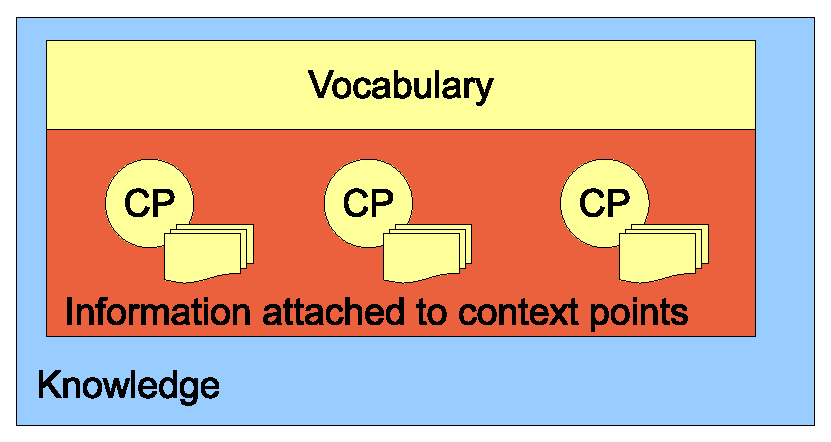
\includegraphics[width=0.40\textwidth]{knowledgecomponents.eps}
\caption{Knowledge components}
\label{fig:knowledgecomponents}
\end{figure}

Context points are means to store information with their coordinates, see previous chapter. Just exchanging sets of context points isn't sufficient in a semantic P2P system. Let's discuss it with an example we already know.

Alice stored information with coordinates: \\
(Shark, Alice, Alice, any, any, any, OUT).

Alice knows more, though. She knows that Shark {\it is a} P2P system. This fact isn't defined with coordinates. It is part of her vocabulary. Alice is willing to transmit information to others -- to Bob in our example. Apparently, it wouldn't be sufficient if she'd send just the context point. She should also send parts of her vocabulary which gives some background information.

In Shark, {\bf knowledge is set of context points with a vocabulary}. Knowledge is rarely created by developers. In most cases it is extracted from a knowledge base. Nevertheless, we want to demonstrate usage of knowledge with a little example.


\begin{verbatim}
SharkVocabulary v = new InMemoSharkKB();
Knowledge k = InMemoSharkKB.createInMemoKnowledge(v);
ContextPoint cp = null; // should not be empty
k.addContextPoint(cp);
SharkVocabulary kVocabulary = k.getVocabulary();
\end{verbatim}

We already know, that a vocabulary can be stored in a knowledge (line 1). There is an in-memory variant of knowledge which can be created with {\tt InMemoSharakKB} which isn't necessary that often in real applications. We use the vocabulary as parameter which becomes part of the knowledge.

We create a context point in line 3. It is empty which is not useful in real applications as well. We can add a context point to the knowledge. Line 4 illustrates the get-method for retrieving the vocabulary from an existing knowledge object.

Figure \ref{fig:knowledgecomponents} illustrates the parts of a knowledge object.


We can now summarise. Each {\tt SharkKB} contains a vocabulary, knowledge and has an owner, see figure \ref{fig:sharkkbcontent}.

\begin{figure}[t]
\centering
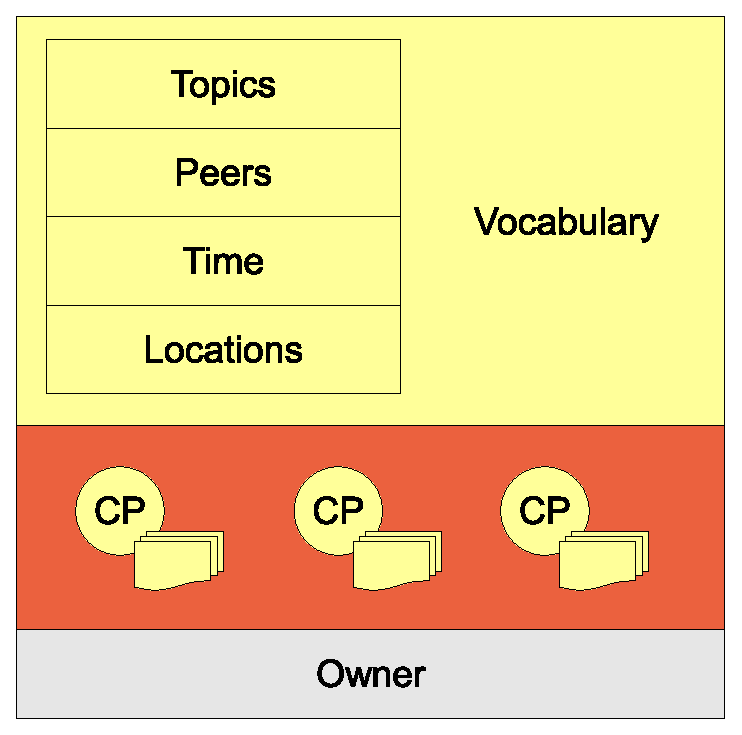
\includegraphics[width=0.50\textwidth]{sharkkbcontent.eps}
\caption{Parts of a Shark KB}
\label{fig:sharkkbcontent}
\end{figure}

\section{Knowledge Extraction}
\label{sec:extraction}
There are two quite complex operations provided by a knowledge base: Extraction and assimilation. We are going to explain both of them and start with extraction. Developers don't have to deal with these operation when using pre-defined knowledge ports. Nevertheless, the basic idea of extraction and assimilation should be understood.

Let's start with an example. (This and the following examples can be found on sharksystem.net under tutorials as {\tt ExtractionAssimilationExamples}.

\begin{verbatim}

this.kb = new InMemoSharkKB();

PeerSemanticTag alice = 
  this.kb.createPeerSemanticTag("Alice", 
       "http://www.sharksystem.net/alice.html", 
       "mail://alice@wonderland.net");

// she owns that kb
this.kb.setOwner(alice);

// create background knowledge
Taxonomy tx = this.kb.getTopicsAsTaxonomy();

// describe programming languages and java as part of a taxonomy
TXSemanticTag pl = tx.createTXSemanticTag("PL",
   "http://en.wikipedia.org/wiki/Programming_language");

TXSemanticTag java = tx.createTXSemanticTag("Java", 
   "http://en.wikipedia.org/wiki/Java_%28programming_language%29");

// move java "under" pl
java.move(pl);
// create two coordinates to fill that kb
ContextCoordinates ccPL = this.kb.createContextCoordinates(
   pl, alice, alice, // topic, originator, peer
   null, null, null, // remote peer, location, time
   SharkCS.DIRECTION_INOUT); / direction

ContextCoordinates ccJava = this.kb.createContextCoordinates(
   java, alice, alice, 
   null, null, null, 
   SharkCS.DIRECTION_INOUT);

ContextPoint cpPL = this.kb.createContextPoint(ccPL);
ContextPoint cpJava = this.kb.createContextPoint(ccJava);

cpPL.addInformation("something about programming languages");
cpJava.addInformation("something about java");

System.out.println("kb after initialisation: ");
System.out.println(L.kbSpace2String(this.kb));
\end{verbatim}

Each code example on the web page create a more or less lengthy output. We reduce the output to a minimum. This program prints out the newly created knowledge base.

\begin{verbatim}
owner: Alice

Vocabulary:
topics: PL->java
peers: Alice

Context Points
#0 (Java, Alice, Alice, any, any, any, inout)
#1 (PL, Alice, Alice, any, any, any, inout)
\end{verbatim}

\begin{figure}[t]
\centering
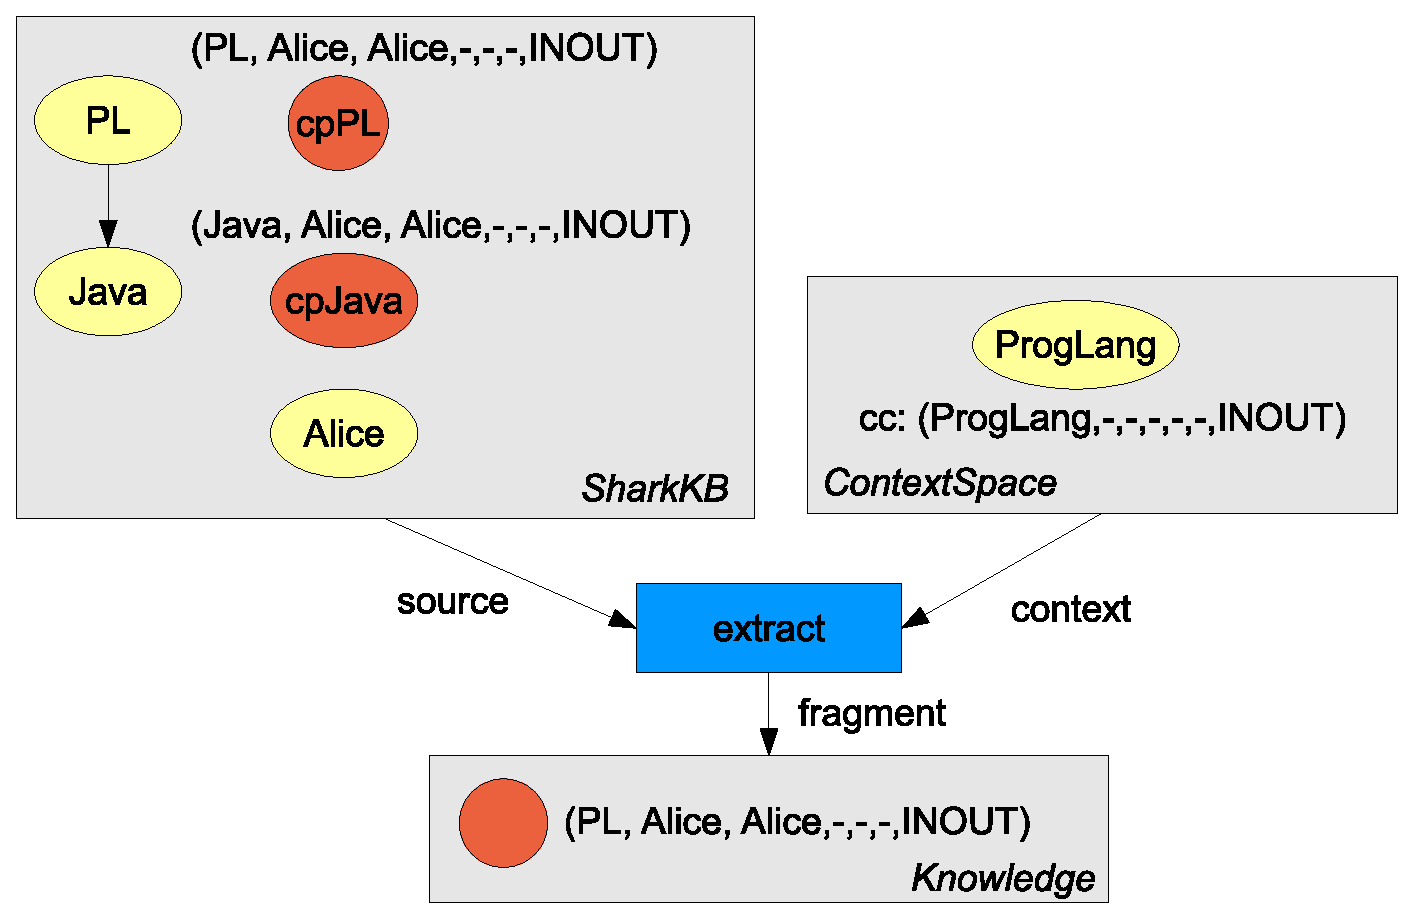
\includegraphics[width=0.60\textwidth]{extraction.eps}
\caption{Extraction example}
\label{fig:extraction}
\end{figure}

The code is not complicated:
An in memory knowledge base is created. Alice is described with a peer semantic tag. Java and programming languages are added to the {\it topic} set in that in our knowledge base. We also describe that Java {\it is a} programming language. Two coordinates are defined and information are added to both points. Both points have Alice as originator and peer. They differ in their topic dimension. One uses Java, the other takes - more general - programming languages as topic. Finally, we print out knowledge base content for debugging purposes. 

Figure \ref{fig:extraction} illustrates most data structures: The {\tt SharkKB} with its three semantic tags and both context points are on the left upper side. 
The tag labeled {\it ProgLang} is on the right side. It is not part of the knowledge base. It just exists in memory.

Let's continue our example with the following code.

\begin{verbatim}
SemanticTag plST = 
   InMemoSharkKB.createInMemoSemanticTag("ProgLang", 
      "http://en.wikipedia.org/wiki/Programming_language");

ContextCoordinates cc = 
   InMemoSharkKB.createInMemoContextCoordinates(
      plST, null, null, null, null, null, 
      SharkCS.DIRECTION_INOUT);

Knowledge k = SharkCSAlgebra.extract(kb, cc);

System.out.println(L.knowledge2String(k.contextPoints()));
\end{verbatim}

We create a single semantic tag describing programming languages. 
We use a different name but the same subject identifier. Thus, this 
tag {\it is identical} to the programming languages tag in our knowledge base.

We create a quite simple coordinate {\tt cc}. We just define the topic dimension. Any other dimension remains {\it any}. We use this coordinate as parameter for the {\tt extract} method. As a result, knowledge is returned with a single point as content and these coordinates:\\

{\tt PL, Alice, Alice, any, any, any, inout}\\

The coordinates are used as template, as query to the knowledge base. Extract looks for any context point that {\it fits} to that template. We use context coordinates in our first examples. {\it Interest} can be used as well. They are more flexible because they can contain more than one tag in each dimension.

Let's have a look on another example:

\begin{verbatim}
PeerSemanticTag aliceTag = 
   InMemoSharkKB.createInMemoPeerSemanticTag(
      "A", 
      "http://www.sharksystem.net/alice.html", 
      null);

ContextCoordinates cc = 
   InMemoSharkKB.createInMemoContextCoordinates(
      null, 
      aliceTag, 
      null, null, null, null, SharkCS.DIRECTION_INOUT);

Knowledge k = SharkCSAlgebra.extract(kb, cc);

System.out.println(L.knowledge2String(k.contextPoints()));

\end{verbatim}

A peer semantic tag is created in the first line. This tag can be seen as
template as well. We have described the subject identifier. Name and address are
more or less undefined. We use this tag as only relevant part to extract knowledge from our knowledge base.

The retrieved knowledge consists of two context point with these coordinates:\\

{\tt java, alice, alice, any, any, any, inout}\\

{\tt programming languages, alice, alice, any, any, any, inout}\\

Apparently, just a single context point in knowledge base fits to the given context. It is the point with topic {\it PL}.

It is time for a first summary. {\tt Extract} is a kind of query interface offered by the Shark knowledge base. The {\it source} must be a {\tt SharkKB}. It contains vocabulary and knowledge. {\it Context} is a kind of query. During extraction, any context point is added to the fragment that {\it fits} to the context. That {\it fitting} was very simple in this example. Context point coordinates must be {\it identical} to their counterparts in the context. Since any tags are identical to all other tags they can be used a joker sign.

There are variants of extraction.

\subsection{Extraction with fragmentation parameter}
Let's start with another example.

\begin{verbatim}
SemanticTag plST = 
   InMemoSharkKB.createInMemoSemanticTag("PL", 
      "http://en.wikipedia.org/wiki/Programming_language");

FragmentationParameter[] fps = 
   new FragmentationParameter[SharkCS.MAXDIMENSIONS];

// set default - don't follow any direction
for(int d = 0; d < SharkCS.MAXDIMENSIONS; d++) {
   fps[d] = FragmentationParameter.getZeroFP();
}

// set topic dimension fragmentation
fps[SharkCS.DIM_TOPIC] = 
   new FragmentationParameter(
      false, // don't follow super tags
      true, // follow sub tags
      1); //depth 1

ContextCoordinates cc = 
   InMemoSharkKB.createInMemoContextCoordinates(
      plST, null, null, null, null, null, 
      SharkCS.DIRECTION_INOUT);

Knowledge k = SharkCSAlgebra.extract(kb, cc, fps);

System.out.println(L.knowledge2String(k.contextPoints()));
\end{verbatim}

We have created our previous example. We create a semantic tag representing programming languages, create coordinates and extract information.
Result of this example both context points instead of a single point as in example one.

Fragmentation parameter make the difference. We have already learned about those parameter in the previous chapter. Tag {\it programming languages} has a single sub tag, namely {\it Java}. In this example, it is defined to follow sub tags but no super tags in topic dimension. No related tags are used in each other dimensions (defined by {\tt zeroFP}. 

We use this array of parameters and use another variant of {\tt extract}. 
\begin{figure}[t]
\centering
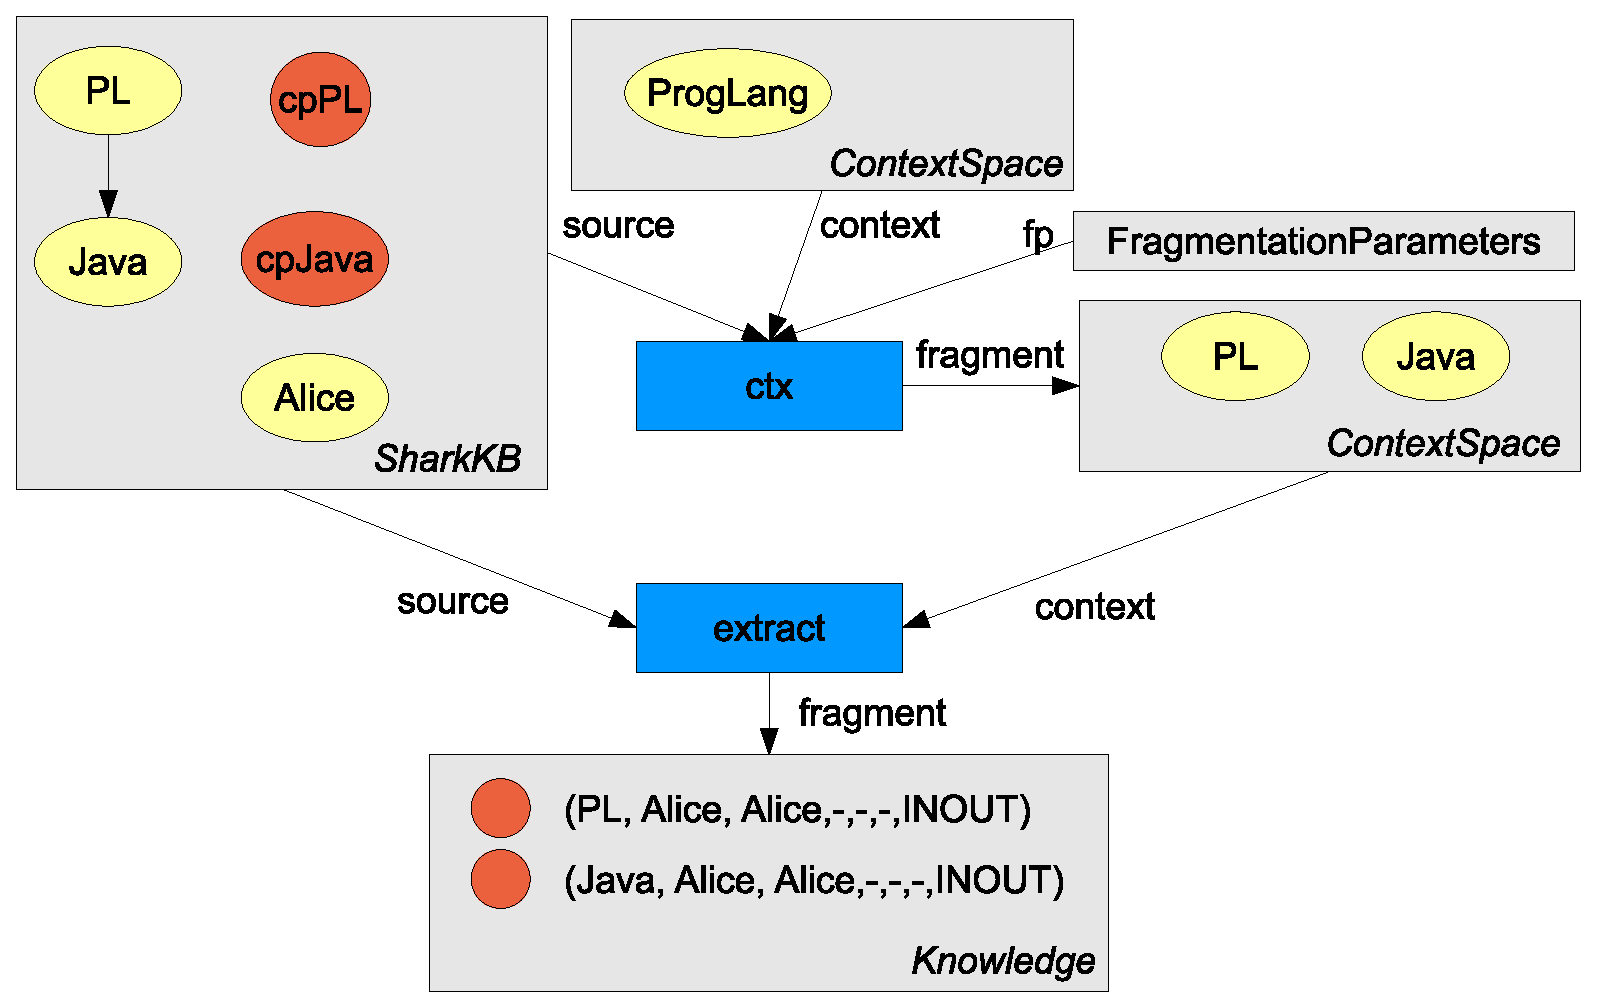
\includegraphics[width=0.60\textwidth]{extractionWithFPs.eps}
\caption{Extraction with fragmentation parameters}
\label{fig:extractionWithFPs}
\end{figure}

Figure \ref{fig:extractionWithFPs} illustrates the process.

\begin{enumerate}
\item A contextualization is made. The first parameter (our knowledge base in this case (and more specific: its vocabulary) is used as source. The second parameter ({\tt cc} in this case) is used as context. That {\tt ContextCoordinate} just contains one real semantic tag which describes programming languages. Fragmentation parameter configure contextualization process. The result is an {\tt SharkCS}. That context space contains two semantic tag on it topic dimension, see figure \ref{fig:extractionWithFPs}. Tag {\it PL} is {\it identical} to anchor {\it ProgLang}. Tag {\it Java} can be reached from {\it PL} under the constraints of fragmentation parameters.

\item The newly calculated context space is taken as context for the final extraction. Apparently, that context covers both context point in our knowledge base. Both are added the resulting knowledge fragment.
\end{enumerate}

This may sound complicated but the idea is simple. Remember our Bob in the early chapters. He is interested in programming languages in general but has no idea about Java. In Shark speech: Java is not part of his vocabulary yet. He can only ask for information of programming languages.

Alice knows about Java and the fact that Java {\it is a} programming language. This variant of {\tt extract} brings both together. Bob is able to describe his interest. Alice could receive that interest and expand it controlled by fragmentation parameter. Finally, she extracts knowledge. 

This knowledge contains more than Bob has asked for. That is a major feature of the Shark framework. Bob can learn content (information) but also semantic tags and their relations.

We conclude this sub section with another example.
\begin{verbatim}

Taxonomy tTax = this.kb.getTopicsAsTaxonomy();
TXSemanticTag plTag = 
   tTax.getSemanticTag(
      "http://en.wikipedia.org/wiki/Programming_language");

TXSemanticTag csharpST = 
   tTax.createTXSemanticTag(
      "c#", "http://cshark.com");

csharpST.move(plTag);

ContextCoordinates ccCSharp = 
   this.kb.createContextCoordinates(
      csharpST, null, null, null, null, null, 
      SharkCS.DIRECTION_INOUT);

ContextPoint cp = this.kb.createContextPoint(ccCSharp);
cp.addInformation("information about c#");

SemanticTag javaST = 
   InMemoSharkKB.createInMemoSemanticTag(
      "Java", 
      "http://en.wikipedia.org/wiki/Java_%28programming_language%29");

FragmentationParameter[] backgroundFPs = 
   new FragmentationParameter[SharkCS.MAXDIMENSIONS];

for(int d = 0; d < SharkCS.MAXDIMENSIONS; d++) {
   backgroundFPs[d] = FragmentationParameter.getZeroFP();
}

backgroundFPs[SharkCS.DIM_TOPIC] = 
   new FragmentationParameter(true, true, 2);

ContextCoordinates cc = 
   InMemoSharkKB.createInMemoContextCoordinates(
      javaST, null, null, null, null, null, 
      SharkCS.DIRECTION_INOUT);

Knowledge k = SharkCSAlgebra.extract(kb, cc, backgroundFPs);
\end{verbatim}

We create another context point with topic {\it cSharp} which is sub tag of {\it programming languages}. We define fragmentation parameters that follows our topic taxonomy in both direction: up to super tags and down to sub tags. We use depth of 2. Extraction anchor is our {\it Java} topic. There are no other constraints. The result contains all three context points.

\subsection{Peer hierarchies}
We extend our program again.

\begin{verbatim}

PeerTaxonomy pTax = this.kb.getPeersAsTaxonomy();

TXSemanticTag alice = 
   pTax.getSemanticTag(
      "http://www.sharksystem.net/alice.html");

PeerTXSemanticTag group = 
   pTax.createPeerTXSemanticTag(
      "Group of Alice", "http://aGroup.org", (String)null);

alice.move(group);

ContextCoordinates groupCC = 
   this.kb.createContextCoordinates(
      null, null, group, null, null, null, 
      SharkCS.DIRECTION_INOUT);

ContextPoint cp = this.kb.createContextPoint(groupCC);

cp.addInformation("information from group");

FragmentationParameter[] backgroundFPs =
   new FragmentationParameter[SharkCS.MAXDIMENSIONS];

for(int d = 0; d < SharkCS.MAXDIMENSIONS; d++) {
   backgroundFPs[d] = FragmentationParameter.getZeroFP();
}

backgroundFPs[SharkCS.DIM_PEER] = 
   new FragmentationParameter(false, true, 1);
//   new FragmentationParameter(false, false, 1);

Knowledge k = SharkCSAlgebra.extract(kb, groupCC, backgroundFPs);
}
\end{verbatim}

We have created a hierarchy as in our previous example but in the peer tag vocabulary.
Alice becomes part of a newly created {\tt group}. The following code is similar. Fragmentation parameter can be used in the same way. The combination 
{\tt false, true} leads to knowledge that is filled with all context points. Try other true/false combinations and watch the results.

\subsection{Cutting peer hierarchies}
Lets review our last example. We have created a context point that has a group in its peer dimension. That's usual and advisable. It is convenient and efficient to create groups and add peers. Afterwords, we can add information and use those groups to define what peers (plural!) shall get these information.

Shark is a P2P system. Each peer can define its own group. Such a group can be compared with recipient list in e-mail. In a number of case, users don't want to reveal neither existence nor members of such a list, though.

This issue can be resolved with our final {\tt extract} variant. We continue our example.

\begin{verbatim}
PeerSemanticTag alice = 
   this.kb.getPeerSTSet().
      getSemanticTag(
         "http://www.sharksystem.net/alice.html");

ContextCoordinates cc = 
   this.kb.createContextCoordinates(
       null, null, alice, null, null, null, 
       SharkCS.DIRECTION_INOUT);

FragmentationParameter[] backgroundFPs = 
   new FragmentationParameter[SharkCS.MAXDIMENSIONS];

for(int d = 0; d < SharkCS.MAXDIMENSIONS; d++) {
   backgroundFPs[d] = FragmentationParameter.getZeroFP();
}

backgroundFPs[SharkCS.DIM_PEER] = 
   new FragmentationParameter(true, true, 1);

Knowledge k = SharkCSAlgebra.extract(kb, cc, backgroundFPs, alice);
\end{verbatim}

This {\tt extract} variant works the same as the previous one at first. It uses fragmentation parameter to find fitting context points. This example will produce again knowledge with four pieces of information. 

The extraction process does not end after context point extraction, though. Peer groups are post-processed: The fourth parameter ({\tt alice} in this case) is called {\it recipient}. Any group peer in context coordinates are removed by the recipient peer. All group peers are also removed from vocabulary. No group peer remains to which Alice belongs to.

We call this process {\it group cutting} and it is used to hide groups in general and member of groups to other peers in particular.

Take care: Groups are only cut if recipient is part of the group. A group cutting is not performed if each of the following cases is true.

\begin{itemize}
\item 
There is a group in a peer dimension of a context point of the extracted knowledge.

\item 
The receiving peer is not member of that group.
\end{itemize}

That situation can only occur when {\it any} tags are involved. Without {\it any} tags, a context point would only become part of the knowledge fragment if the context fits to its coordinates. {\it Fitting} means, it semantic tags are either identical or part of a group. Cutting will hide any group from remote peers automatically.

Problems may arise if unidentified peers are accepted as receiver. The remote peer is described with an {\it any} tag in that case. That tag fits to each peer but also to each peer group. Group cutting cannot be performed because identity of receiver is unknown. That special case can be handled when writing own knowledge port.

Using group hierarchies and {\it any} tags together can become a bit tricky. Take care!

\section{Knowledge Assimilation}
Whenever we talk about information and knowledge, we have to consider who created information and who shall be recipient.

Extraction is used to produce a bunch of information combined with a vocabulary to send both to another peer. Any peer is allowed to send knowledge to any peer under any circumstances.

A peer that receives knowledge has to consider several issues.

\begin{enumerate}
\item 
Am I willing to receive any information from that peer?
\item 
What topic am I'm interested in? More general, what general constraints do I have when receiving information?
\item 
What dedicated information should I store?
\end{enumerate}

That process is called {\it assimilation}\footnote{Yes, the word is stolen from the Borg which play a quite relevant role in Star Trek.} in Shark. It starts when knowledge has been received. Peers are free in its reaction to incoming knowledge. In most cases, peers store information in which they are interested in. For such applications, the following section can be helpful.

Have a look at {\it example8} which can be found under {\it Knowledge Base Examples} on our web 
site\footnote{http://www.sharksystem.net/codeExamples/sharkkb.zip}.

First lines in that example create a knowledge object that contains 
two points:

\begin{verbatim}
(Java, Alice, Alice,-,-,-, inout)
(PL, Alice, Alice,-,-,-, inout)
\end{verbatim}

Let's see what happens afterwords in this example:

\begin{verbatim}
Knowledge k = ... // contains two cp now.
FragmentationParameter[] backgroundFPs = .. //zeroFP

//lets start with assimilation
STSet t = InMemoSharkKB.createInMemoSTSet();

// create java tag template
t.createSemanticTag(null, 
   "http://en.wikipedia.org/wiki/Java_%28programming_language%29");

// create interest as filter for assimilation
Interest i = InMemoSharkKB.createInMemoInterest(
   t, null, null, null, null, null, 
   SharkCS.DIRECTION_INOUT);

// create empty kb
SharkKB kb1 = new InMemoSharkKB();

// fill new kb with learning and no removing
SharkCSAlgebra.assimilate(kb1, i, 
   backgroundFPs, k, true /*learn*/, 
   false/* remove cp */);

System.out.println(L.kb2String(kb1));

\end{verbatim}

A semantic tag is created that has no name but an identity. Is represents {\it programming languages}. An interest is created that contains just that tag.

An empty knowledge base ({\tt kb1}) is created. Afterwords, the assimilation is started and uses the empty knowledge base as target and the knowledge as source. 
{\tt backgroundFP} is a zero parameter set - depth is zero in each dimension.

\begin{figure}[t]
\centering
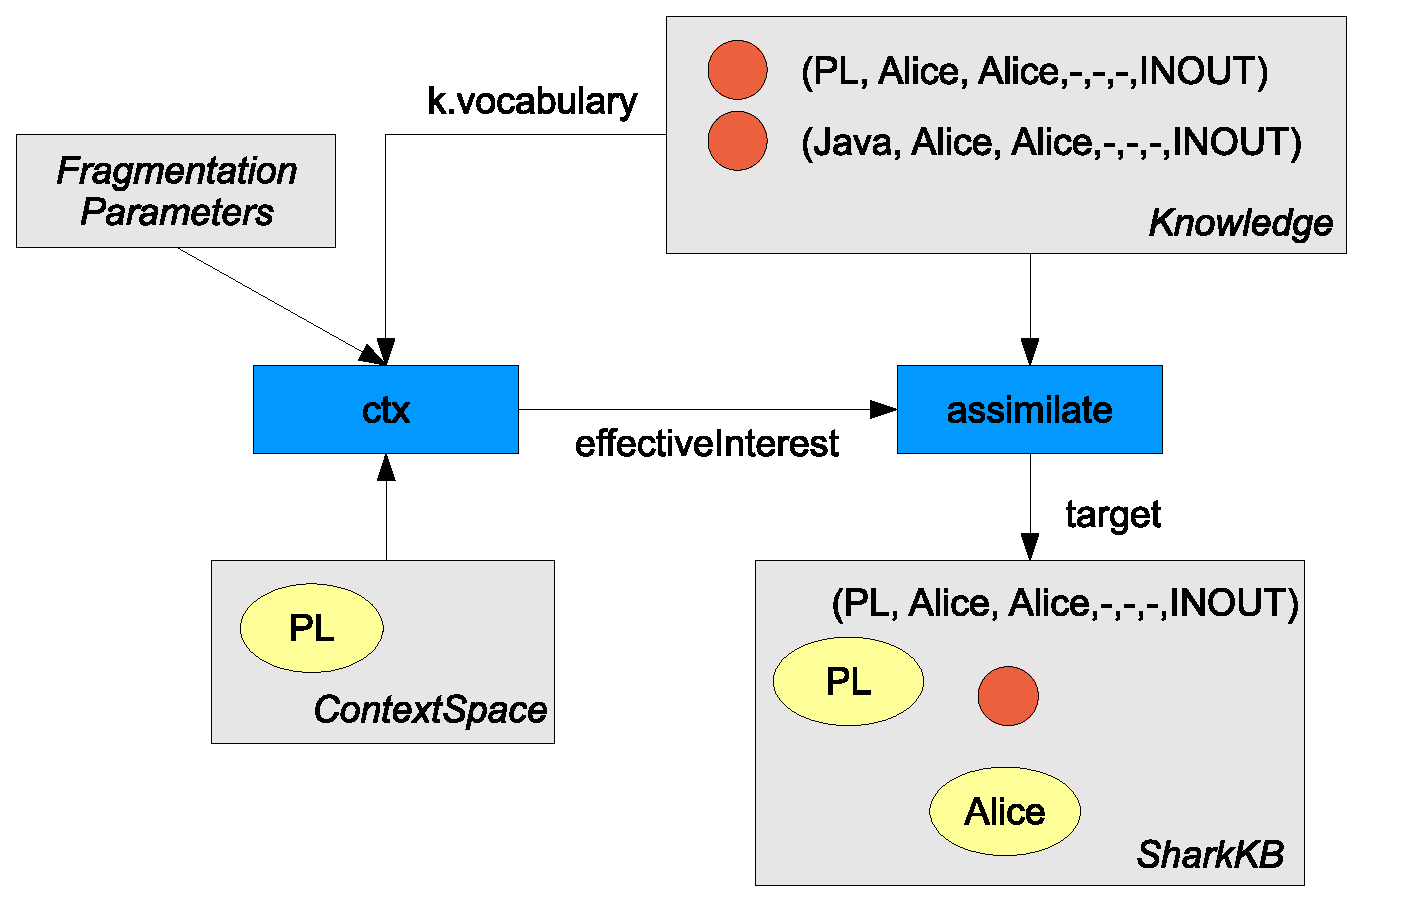
\includegraphics[width=0.70\textwidth]{assimilation.eps}
\caption{Assimilation}
\label{fig:assimilation}
\end{figure}

Figure \ref{fig:assimilation} illustrates the process. It consists on two general steps.

\begin{enumerate}
\item 
A contextualization is performed, see left side in figure \ref{fig:assimilation}. Knowledge vocabulary is taken is source. The interest serves as context and the fragmentation parameter are the third parameter. The result is called {\it effective interest}. What is that good for?

Vocabulary of sender and receiver might differ. Thus, there can be tags in knowledge which are unknown to recipient. The receiving peer has a chance to learn tags in this step. It defines anchor and fragmentation parameter. 

Receiver isn't interested in our example code. Fragmentation parameter are {\it zero parameter} in each dimension. In that case, contextualization is simple: Each tag that is in receiver's interest and the knowledge vocabulary is also part of the {\it effective interest}.

\item 
As we could see, an interest spans a context space. So does the {\it effective interest}. It covers a space which is of interest of receiving peer. Now, each context point in knowledge is added to the target knowledge base which is in this space. All other context points are ignored.
\end{enumerate}

Content of kb1 after assimilation is this:

\begin{verbatim}
Vocabulary:
topics: Java
peers: Alice
Content:
#0: (PL, Alice, Alice, any, any, any, inout)
\end{verbatim}

Seems to be pretty obvious. We have learned about Java and Alice and both words are added to our vocabulary\footnote{and brought us closer to perfection. I couldn't hesitate to frame with phrases from the Borg queen.}. Two context points are added as well.

Have a closer look at the assimilated context point. Alice is in the {\it remote peer} dimension and not any longer in the {\it peer} dimension.

It is assumed that knowledge from another peer is assimilated. Thus, we have to change perspective. The remote peer would pronounce itself as peer. The recipient would recognize it as {\it remote} peer, though. Moreover, a peer can declare information to be sent. Now, those information are received. We cannot assume that the peer will also think that those information have to be transmitted immediately. Assimilation makes some changes in dimensions:

\begin{itemize}
\item Peer and remote peer dimension change places.
\item Direction is changed. OUT and INPUT becomes IN. NOTHING remains unchanged. Direction IN wouldn't be accepted anyway because it wouldn't match to an receiving interest.
\end{itemize}

There are two parameter left to be explained. Let's start with the easy one: 
{\tt deleteAssimilated} is a boolean value. Set to {\tt true} each context point that was assimilated is removed from knowledge. Applications which use a single knowledge base should always use the {\tt true} setting. That avoids re-assimilation of same knowledge by different knowledge ports. It makes no sense to add knowledge twice. Once added to the local knowledge base it can be removed. Following knowledge port has less to do. Applications with more than one knowledge base will have probably another strategy.

They {\tt learnTags} parameter is a boolean value. A peer learns vocabulary from received knowledge if set {\tt true}. The local vocabulary will remain unchanged otherwise. How could a peer learn vocabulary?

Review our last example. Knowledge arrived with two context points. One is about {\it Java}, the other about {\it programming languages}. The effective interest contained only {\it programming languages} due to the zero fragmentation parameter. 

Lets assume, we have had chosen a more broader parameter set. Maybe we have allowed to extract related tags to {\it programming languages}. In this case, {\it Java} would have become part of effective interest and second context point would have been added to the local knowledge base. If {\tt learnTags} would be set to true, {\tt kb1} would contain two points then:

\begin{verbatim}
(Java, Alice, Alice,-,-,-, inout)
(PL, Alice, Alice,-,-,-, inout)
\end{verbatim}

Receiver would have learned tag {\it Java} and two context points are added.

Just a single context point would exists after assimilation if {\tt learnTags} would have set to {\tt false}: 

\begin{verbatim}
(PL, Alice, Alice,-,-,-, inout)
\end{verbatim}

No {\it Java} tag would have be learned. But note, the second context was assimilated as well! We haven't changed anything on fragmentation parameter. What happened?

Assimilation algorithm decides whether a context point gets added to the local knowledge base or not. That decision is made independently if tags are to be learned or not. There can be context points which have tags in their dimensions which are unknown in the local vocabulary. Such tags are replaced by the closest locally known tags.

In our example, the receiving peer refused to learn the tag {\it Java}. The closest tag to {\it Java} is {\it programming languages}. Thus, all information are added to the context point as well.

When running the program, you'll see that {\tt (PL, Alice, Alice,-,-,-, inout)}
has two attached information.

That's it. We won't discuss any method from {\tt SharkKB}. Most of them are pretty obvious. We strongly recommend to make the exercises. They help to understand the concept. And they are not that difficult. Solutions can be found on the sharksystem.net web page. But it's better making them alone. Good luck!

\section{Exercises}
